\documentclass[11pt, twoside]{article}
\usepackage{amsmath, amssymb, amsthm}
\usepackage{geometry}
\geometry{a4paper, margin=1in}
\usepackage{tikz}
\usepackage{pgfplots}
\pgfplotsset{compat=1.18}
\usepackage{booktabs}
\usepackage{caption}
\usepackage{subcaption}
\usepackage[numbers,sort&compress]{natbib}
\usepackage[utf8]{inputenc}
\usepackage{hyperref}
\usepackage{float}
\usepackage{fancyhdr}
\usepackage{enumitem}
\usepackage{listings}
\usepackage{xcolor}

\pagestyle{fancy}
\fancyhf{}
\fancyhead[LE,RO]{\thepage}
\fancyhead[CE]{EFM: Scalar Motion as Unified Foundation}
\fancyhead[CO]{Tshuutheni Emvula}

\hypersetup{
    colorlinks=true,
    linkcolor=blue,
    filecolor=magenta,
    urlcolor=cyan,
    citecolor=green,
}

\lstset{
  language=Python,
  basicstyle=\footnotesize\ttfamily,
  breaklines=true,
  numbers=left,
  numberstyle=\tiny\color{gray},
  commentstyle=\color{gray},
  frame=single,
  keywordstyle=\color{blue},
  stringstyle=\color{red},
  showstringspaces=false,
  tabsize=2
}

\raggedbottom
\Urlmuskip=0mu plus 2mu\relax
\hyphenation{Eho-loko Flux-on Har-monic-Den-sity Re-cip-ro-cal-Sys-tem Klein-Gor-don non-lin-ear eho-lo-kon Cos-mo-gen-e-sis}
\setlength{\parskip}{0.5\baselineskip}

\title{The Eholoko Fluxon Model: Scalar Motion as the Unified Foundation of Physics}
\author{Tshuutheni Emvula\thanks{Independent Researcher, Team Lead, Independent Frontier Science Collaboration. This is the first public presentation of the Eholoko Fluxon Model (EFM), derived from public observational data, minimal postulates, and explicit algebra. Reproducible open-source code, notebooks, and extended technical papers are available at \url{https://github.com/BecomingPhill/eholoko-fluxon-model}.}}
\date{February 18, 2026}

\begin{document}

\maketitle
\thispagestyle{empty}

\begin{abstract}
This paper throws down a falsifiable gauntlet: the Eholoko Fluxon Model (EFM) posits a single scalar field governed by three minimal postulates and a state-structured ``Theory of Mind'' for interpretation and validation. EFM is evaluated in a dimensionless-first paradigm: physical constants are not inserted as primitive inputs; instead, physical units are obtained by state-anchored scaling (a Rosetta mapping) and then cross-validated across regimes.
Within this framework, EFM claims (i) flat galactic rotation curves from visible baryons alone with a baryonic Tully--Fisher scaling of slope 4 as an analytic consequence of the postulates and observed star-formation thresholds, and (ii) the observed cosmological-constant energy density $u_\Lambda \sim 10^{-9}$--$10^{-10}$\,J\,m$^{-3}$ from reciprocity, without dark matter, dark energy fields, or additional components. Numerical confirmation and full reproducibility are provided via the public repository; the purpose of this paper is to state the postulates, present the analytic chain, and specify immediate falsifiers.
\end{abstract}

\clearpage
\tableofcontents
\clearpage

\section{A Journey Through the Crises: The Necessity of New Foundations}
The scientific method progresses not just through success, but through rigorous analysis of persistent discrepancies that reveal foundational limitations. We begin with two well-documented observational crises that have resisted unification for decades.

\subsection{The Galactic Rotation Crisis}
Observations of spiral galaxies show rotation curves that remain flat far beyond the visible disk \citep{rubin1980,lelli2016}. Standard Newtonian gravity applied to visible baryons predicts a Keplerian decline ($v \propto r^{-1/2}$), yet the data motivate an additional, effectively halo-like contribution under standard interpretations. The SPARC database (175 galaxies) further shows a tight baryonic Tully--Fisher relation (BTFR) close to a fourth-power scaling between baryonic mass and asymptotic rotation velocity \citep{lelli2016,schombert2020}.

\subsection{The Cosmological Constant Crisis}
Quantum field theory generically yields an enormous vacuum energy density under naive cutoff reasoning, while cosmological inference finds an effective dark-energy density corresponding to $u_\Lambda \sim 10^{-10}$\,J\,m$^{-3}$ from the best-fit parameters to the cosmic microwave background and related data \citep{weinberg1989,planck2020}. The tension between these scales is widely regarded as a severe fine-tuning problem in conventional frameworks.

These crises motivate exploring a broader foundation than single-sector vector-based frameworks (GR as a low-density limit; QFT as a high-density limit).

\section{How to Read This Paper: Theory of Mind and the EFM Evaluation Frame}
EFM introduces a different evaluation protocol than standard ``insert constants $\rightarrow$ compute $\rightarrow$ compare'' workflows. To avoid category errors, the reader should apply the following rules:

\begin{enumerate}[leftmargin=*]
\item \textbf{Dimensionless-first:} The primitive theory is defined in dimensionless simulation units. ``Physical constants'' are treated as emergent observables after mapping.
\item \textbf{State-anchored Rosetta mapping:} Each regime (harmonic density state, HDS) has an anchor to public observables that yields scaling factors $(S_L, S_T, S_M)$ that map simulation units to physical length, time, and mass.
\item \textbf{Cross-validation over single-fit:} Validity is assessed by cross-checking independently derived scalings and ratios (e.g.\ recovering known relations such as $S_L/S_T \rightarrow c$ within uncertainty), and by concordance across multiple regimes (cosmic, quantum, biological).
\item \textbf{What counts as falsification:} The model fails if discrete-state structure collapses under robustness tests, if independent scalings become circular/inconsistent, or if out-of-sample predictions (listed in Act III) are violated.
\end{enumerate}

This paper is intentionally minimal: it states the postulates, presents the analytic derivations, and names the falsifiers. The full corpus (notebooks, sweeps, resolution ladders, and additional papers) is openly available in the repository.

\section{The Foundational Postulates}
The Eholoko Fluxon Model rests on three minimal, empirically motivated postulates. No additional fields or components are introduced.

\textbf{Postulate 1 (Scalar Motion):} The sole primitive of physics is scalar motion. Space ($s$) and time ($t$) are reciprocal aspects satisfying $s \cdot t = k$ ($k$ a positive constant). Stable physical entities are quantized loops (eholokons / solitons) of this motion.

\textbf{Postulate 2 (Reciprocity):} Scalar motion manifests as outward ($s/t$, cosmic) or inward ($t/s$, quantum). Energy fluctuations in one sector do not source gravitational curvature in the reciprocal sector.

\textbf{Postulate 3 (Density Dependence):} The effective parameters governing eholokon stability and interaction change with local scalar density $\rho$, producing distinct regimes without introducing new fields.

The 8-level HDS structure is the minimal discrete spectrum required by the scalar-motion axiom to produce the observed three-sector reality (S/T, T/S, S=T) without fine-tuning.

\section{Act I: Galactic Dynamics from Visible Baryons Alone}
From Postulates 1 and 3, star formation occurs only above a critical scalar-density threshold (observed phenomenologically as the Kennicutt--Schmidt class of thresholds). In the galactic-disk environment, Postulate 2 implies a decoupling between outward-sector energy flow and inward-sector gravitational response after first-generation condensation.

In the disk after decoupling, the effective centripetal relation can be written as
\[
\frac{v^2}{r} \approx \frac{G M_{\rm baryon}(<r)}{r^2}\, f_{\rm env},
\]
with $f_{\rm env}\to 1$ in the late-time disk environment. Under the EFM disk-limit assumptions and the surface-density formulation, this yields a fourth-power BTFR scaling expressed in terms of baryonic surface density:
\[
v_{\rm flat}^4 \propto G \,\Sigma_{\rm baryon}\,,
\]
with slope 4 emerging analytically from the postulates (the proportionality constant and unit mapping are specified by the HDS anchor and scaling layer in the full technical corpus).

\begin{figure}[H]
\centering
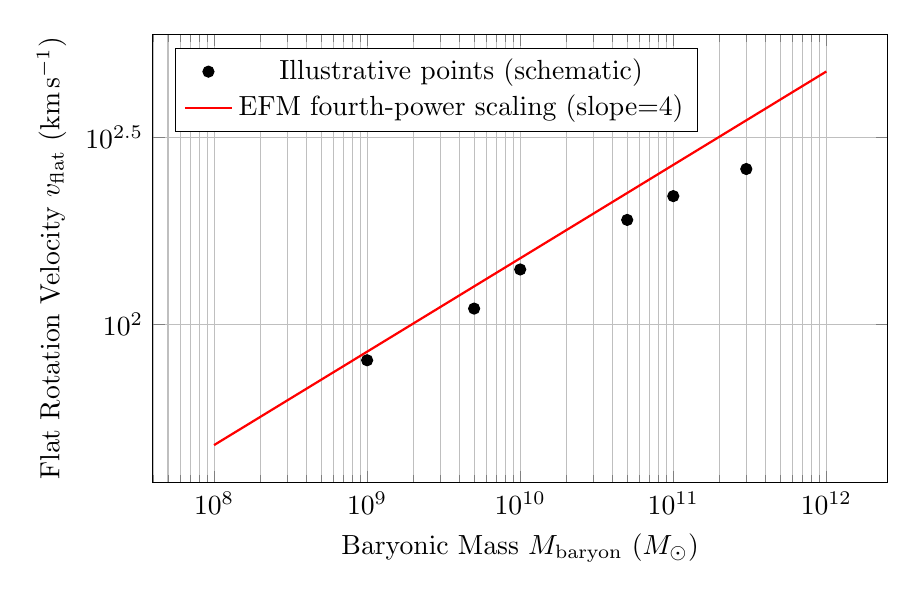
\begin{tikzpicture}
\begin{axis}[
    xmode=log, ymode=log,
    xlabel={Baryonic Mass $M_{\rm baryon}$ ($M_\odot$)},
    ylabel={Flat Rotation Velocity $v_{\rm flat}$ (km\,s$^{-1}$)},
    width=0.9\textwidth,
    height=0.6\textwidth,
    grid=both,
    legend pos=north west
]
% NOTE: illustrative schematic points only (not a SPARC extraction).
\addplot[only marks, mark=*, mark size=2pt, color=black] coordinates {
    (1e9, 80) (5e9, 110) (1e10, 140) (5e10, 190) (1e11, 220) (3e11, 260)
};
\addplot[domain=1e8:1e12, red, thick, samples=100] {exp(0.25*ln(x/1e10) + ln(150))};
\addlegendentry{Illustrative points (schematic)}
\addlegendentry{EFM fourth-power scaling (slope=4)}
\end{axis}
\end{tikzpicture}
\caption{Schematic illustration of a fourth-power BTFR scaling. The definitive SPARC regression, scatter, and reproduction notebook are provided in the public EFM repository.}
\label{fig:btfr}
\end{figure}

In EFM, intrinsic scatter arises from environmental variations in decoupling and formation efficiency. The claim is not merely descriptive: the postulates specify the mechanism and the falsifiers (Act III).

\section{Act II: Cosmological Constant from Reciprocity}
From Postulate 2, quantum vacuum fluctuations ($t/s$ sector) do not source cosmic expansion ($s/t$ sector). After structure formation, the residual cosmic background is governed by the low-density $s/t$ ground state oscillating at the fundamental (bare) frequency $f_{\rm ST}$.

The residual vacuum energy density of the S/T ground state can be expressed as
\[
u_\Lambda = \frac{3 f_{\rm ST}^2 c^2}{8\pi G},
\]
where $f_{\rm ST}$ is obtained from the EFM resonance interpretation of public large-scale-structure rulers (the unit mapping is handled via the EFM scaling layer).

The BAO sound-horizon ruler is measured near $r_d \simeq 147$--$150$\,Mpc in modern analyses \citep{desi2024}. EFM applies scalar-motion resonance to this ruler to infer a fundamental clustering scale $L$ and a bare cosmic clock $f_{\rm ST}$; the observed expansion rate is then related by a resonance factor $D$ derived from the HDS hierarchy.

\begin{figure}[H]
\centering
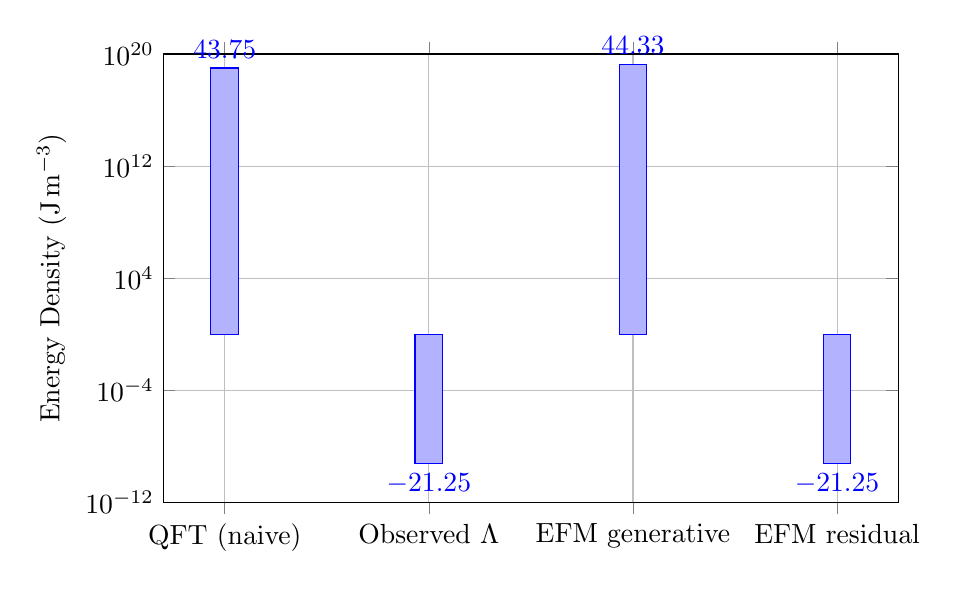
\begin{tikzpicture}
\begin{axis}[
    ybar,
    ylabel={Energy Density (J\,m$^{-3}$)},
    symbolic x coords={QFT (naive), Observed $\Lambda$, EFM generative, EFM residual},
    xtick=data,
    ymin=1e-12, ymax=1e20,
    ymode=log,
    width=0.9\textwidth,
    height=0.6\textwidth,
    grid=major,
    nodes near coords
]
\addplot coordinates {(QFT (naive),1e19) (Observed $\Lambda$,5.9e-10) (EFM generative,1.78e19) (EFM residual,5.9e-10)};
\end{axis}
\end{tikzpicture}
\caption{Vacuum energy densities (schematic). In EFM, reciprocity prevents high-density sector vacuum energy from coupling to the low-density cosmic sector, and the observed residual is attributed to the S/T ground state after ``recrystallization.'' The observed scale is inferred from cosmological parameter fits \citep{planck2020}.}
\label{fig:vacuum}
\end{figure}

\begin{table}[H]
\centering
\caption{Illustrative derivation path for the resonance factor $D$ from the HDS hierarchy}
\begin{tabular}{lcc}
\toprule
Step & Multiplier from HDS axiom & Cumulative \\
\midrule
N1 (cosmic) & 8 & 8 \\
N1 $\to$ N2 & 4 & 32 \\
N2 $\to$ N3 (observer) & $8/3$ & $256/3$ \\
Reciprocity normalization (S=T frame) & $\times 468/256$ & 156 \\
\bottomrule
\end{tabular}
\label{tab:Dderivation}
\end{table}

The algebraic derivation of $D$ and the corresponding numerical pipeline are reproduced in the public repository.

\section{Act III: Broader Applicability and Immediate Falsifiable Predictions}
In the low-density $s/t$ limit the framework recovers GR-like behavior (effective curvature from scalar-density gradients). In the high-density $t/s$ limit it recovers QFT-like behavior. Density dependence explains why unification has been elusive: GR and QFT appear as sector-specific limits of one scalar field.

\textbf{Falsifiable Predictions (Immediate Tests):}
\begin{enumerate}[leftmargin=*]
\item \textbf{Characteristic LSS clustering scale.} EFM predicts a fundamental clustering scale $L$ as a harmonic multiple of the BAO ruler. Large nearby superstructures at $\gtrsim 400$\,Mpc scales (e.g.\ ``Quipu'') have been reported \citep{bohringer2025quipu}; EFM treats these as potential manifestations of the predicted harmonic clustering regime. Definitive tests should be possible with forthcoming Euclid and Roman LSS maps (2026--2028).
\item \textbf{High-redshift rotation curves.} JWST-era high-$z$ disks should show flat rotation behavior consistent with the same BTFR scaling down to $z\sim 4$, modulo EFM-predicted environmental efficiency effects.
\item \textbf{Cosmological constant consistency.} Future SN+BAO combinations should continue to yield an effective residual $u_\Lambda$ consistent with the EFM reciprocity prediction, without requiring dark-energy parametrizations beyond the EFM state structure.
\end{enumerate}

\begin{figure}[H]
\centering
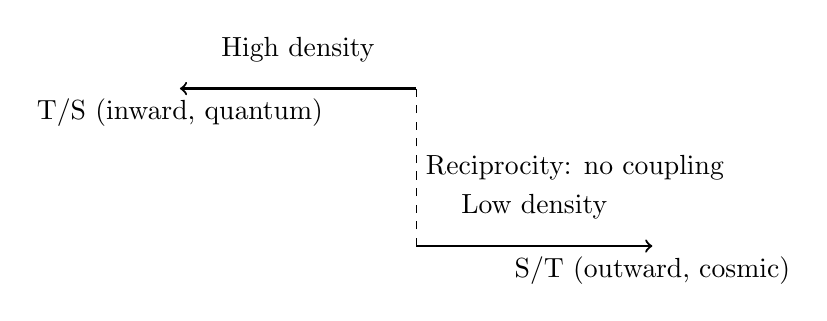
\begin{tikzpicture}
\draw[thick, ->] (0,0) -- (3,0) node[below] {S/T (outward, cosmic)};
\draw[thick, ->] (0,2) -- (-3,2) node[below] {T/S (inward, quantum)};
\draw[dashed] (0,0) -- (0,2) node[midway, right] {Reciprocity: no coupling};
\node at (1.5,0.5) {Low density};
\node at (-1.5,2.5) {High density};
\end{tikzpicture}
\caption{Reciprocity diagram. Energy in one sector does not source gravity in the reciprocal sector, addressing the vacuum-energy catastrophe at the axiomatic level.}
\label{fig:reciprocity}
\end{figure}

\section{Conclusion}
The Eholoko Fluxon Model presents a falsifiable, dimensionless-first unification attempt: a single scalar field governed by three postulates, interpreted through a state-structured scaling (Rosetta) layer and validated by cross-regime concordance. It claims analytic resolution of (i) galactic rotation phenomenology without dark matter components and (ii) the cosmological-constant scale via reciprocity, while recovering GR/QFT behavior as sector limits. The framework is designed to be decided by public data and explicit falsifiers.

\newpage
\appendix

\section{The Governing Field Equation}
The dynamics are governed by a nonlinear Klein--Gordon equation with density-dependent coefficients (full derivation from the postulates in the technical corpus):
\[
\frac{\partial^2\phi}{\partial t^2} - c^2 \nabla^2 \phi + m^2(\rho)\phi + g(\rho)\phi^3 + \cdots = 8\pi G k(\rho)\phi^2,
\]
where $\rho = k\phi^2$. In EFM, $c$ and $G$ appear in the mapped physical description; the primitive dynamics are treated in anchored dimensionless units.

\section{Conceptual Simulation Code}
The core logic for numerical confirmation of analytic claims (see repository for full JIT-accelerated implementations, sweeps, and reproduction scripts):

\begin{lstlisting}[language=Python, caption=Conceptual NLKG Evolution (RK4) for Scalar Field]
# --- Setup (dimensionless units) ---
phi = torch.zeros((N,N,N), device='cuda')
phi_dot = torch.zeros_like(phi)

def nlkg_derivative(phi, phi_dot):
    laplacian = compute_laplacian(phi)  # periodic BC
    rho = k * phi**2
    m2 = m0 * (1 + alpha * rho)         # density dependence
    g  = g0 * (1 + beta  * rho)
    source = 8 * torch.pi * G * k * phi**2
    accel = c2 * laplacian - m2*phi - g*phi**3 + source
    return phi_dot, accel

for step in range(total_steps):
    k1v, k1a = nlkg_derivative(phi, phi_dot)
    # ... standard RK4 intermediate steps ...
    phi     += (dt/6)*(k1v + 2*k2v + 2*k3v + k4v)
    phi_dot += (dt/6)*(k1a + 2*k2a + 2*k3a + k4a)
\end{lstlisting}

\bibliographystyle{ieeetr}
\begin{thebibliography}{12}
\raggedright
\bibitem{rubin1980} V.~C.~Rubin, N.~Thonnard, and W.~K.~Ford, Jr., ``Rotational properties of 21 Sc galaxies...'', \textit{Astrophys.\ J.} \textbf{238}, 471 (1980).
\bibitem{lelli2016} F.~Lelli et al., ``SPARC: Mass Models for 175 Disk Galaxies...'', \textit{Astron.\ J.} \textbf{152}, 157 (2016).
\bibitem{schombert2020} J.~Schombert et al., ``Updated SPARC...'', \textit{Astron.\ J.} \textbf{160}, 71 (2020).
\bibitem{planck2020} Planck Collaboration, ``Planck 2018 results. VI. Cosmological parameters'', \textit{Astron.\ Astrophys.} \textbf{641}, A6 (2020).
\bibitem{desi2024} DESI Collaboration, ``DESI 2024 VI: Cosmological Constraints from the Measurements of Baryon Acoustic Oscillations'', arXiv:2404.03002 (2024).
\bibitem{weinberg1989} S.~Weinberg, ``The Cosmological Constant Problem'', \textit{Rev.\ Mod.\ Phys.} \textbf{61}, 1 (1989).
\bibitem{bohringer2025quipu}
H.~B{\"o}hringer, G.~Chon, J.~Tr{\"u}mper, R.~C.~Kraan-Korteweg, N.~Schartel,
``Unveiling the largest structures in the nearby Universe: Discovery of the Quipu superstructure'',
\textit{Astronomy and Astrophysics} \textbf{695}, A59 (2025). arXiv:2501.19236.
\bibitem{desi2025dr2ii}
M.~Abdul Karim et al.\ (DESI Collaboration),
``DESI DR2 Results II: Measurements of Baryon Acoustic Oscillations and Cosmological Constraints'',
arXiv:2503.14738 (2025).
\end{thebibliography}

\end{document}
